\documentclass[12pt]{article}
\usepackage[utf8]{inputenc} % For UTF-8 encoding
\usepackage{amsmath, amssymb, amsthm} % For mathematical formatting
\usepackage{multirow} % For multirow in tables
\usepackage[a4paper, margin=0.75in]{geometry} % For setting page size and margins
\usepackage{xcolor, listings} % For code highlighting
\usepackage{longtable} % For long tables
\usepackage{graphicx} % For including images
\setlength{\parindent}{0pt}


\title{Computer Architecture HW 3}
\author{111062117, Hsiang-Sheng Huang}

\begin{document}

\maketitle

\section*{1}
\begin{center}
\begin{tabular}{|c|c|c|c|}
\hline
\textbf{$A_{\text{invert}}$} & \textbf{$B_{\text{negate}}$} & \textbf{Operation} & \textbf{Function} \\
\hline
0 & 1 & 11 & add-ext\\
\hline
0 & 0 & 11 & sub-ext \\
\hline
\end{tabular}
\end{center}

\begin{center}
\begin{table}[h]
\centering
\begin{tabular}{|c|}
\hline
\textbf{Complete 64-bit ALU Architecture} \\
\hline
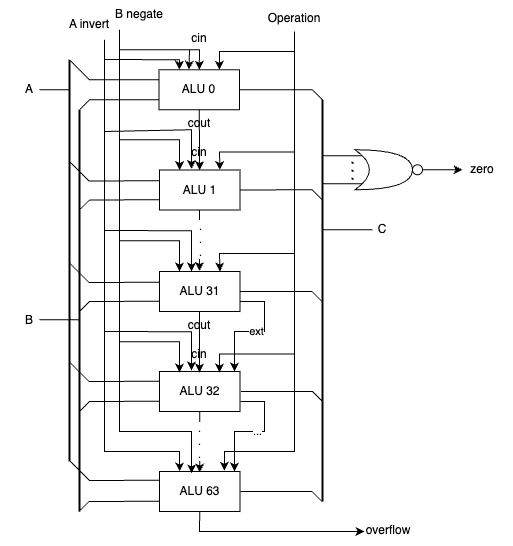
\includegraphics[width=0.84\textwidth]{./img/q1_ALU.png} \\
\hline
\end{tabular}
\end{table}
\end{center}

\begin{center}
    \begin{table}[h]
        \centering
        \begin{tabular}{|c|c|}
            \hline
            \textbf{ALU0} & \textbf{ALU1\textasciitilde 30} \\
            \hline
            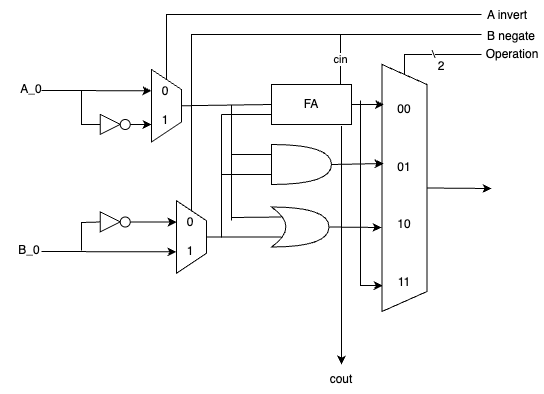
\includegraphics[width=0.42\textwidth]{./img/q1_bit0.png} & 
            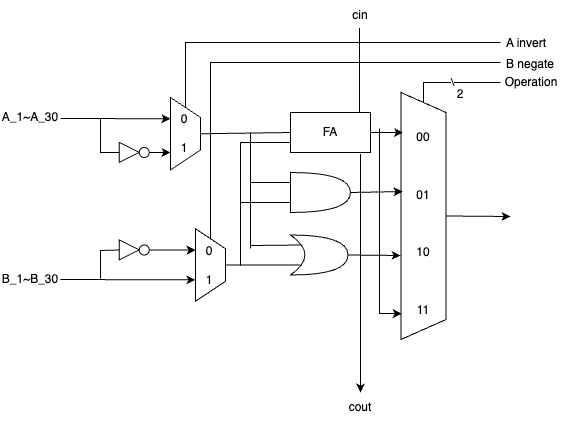
\includegraphics[width=0.42\textwidth]{./img/q1_bit1-30.png} \\
            \hline
            \textbf{ALU31} & \textbf{ALU32\textasciitilde 62} \\
            \hline
            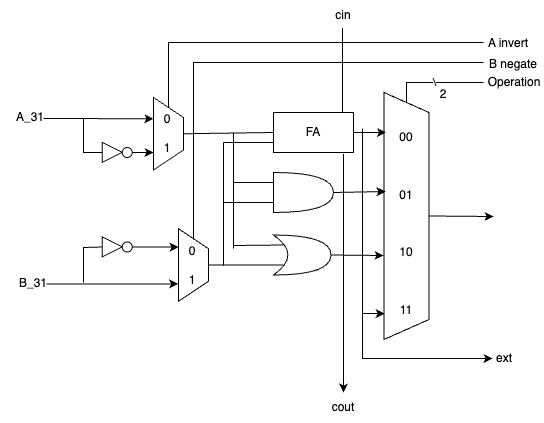
\includegraphics[width=0.42\textwidth]{./img/q1_bit31.png} &
            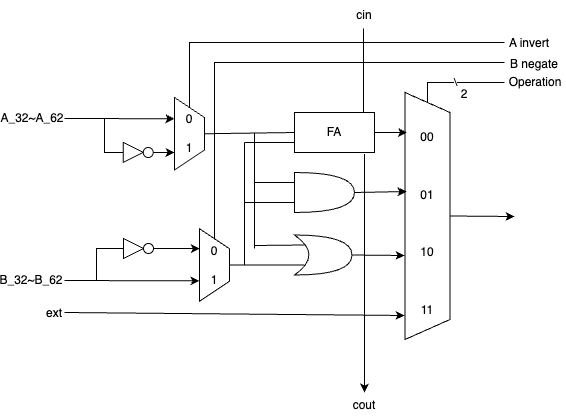
\includegraphics[width=0.42\textwidth]{./img/q1_bit32-62.png} \\
            \hline
            \multicolumn{2}{|c|}{\textbf{ALU63}} \\
            \hline
            \multicolumn{2}{|c|}{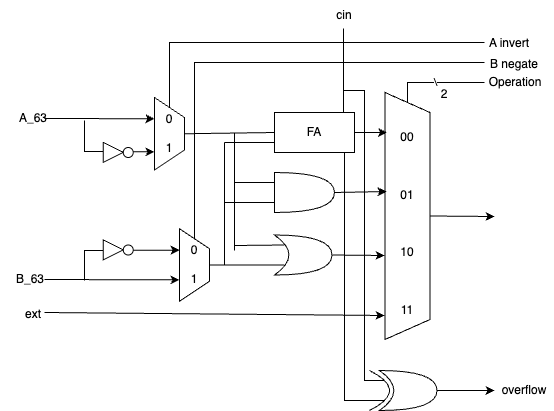
\includegraphics[width=0.42\textwidth]{./img/q1_bit63.png}} \\
            \hline
        \end{tabular}
    \end{table}
\end{center}

\clearpage

\section*{2}

\subsection*{(a)}

\begin{table}[h!]
    \centering
    \begin{tabular}{|c|c|c|c|c|}
    \hline
    \textbf{Iteration} & \textbf{Step} & \textbf{Multiplier} & \textbf{Multiplicant} & \textbf{Product}  \\
    \hline
    0 & Initial Values                 & 1010                & 0000\ 1100            & 0000\ 0000        \\
    \hline
    \multirow{3}{*}{1} 
     & $0\rightarrow\texttt{No operation}$ & 1010            & 0000\ 1100            & 0000\ 0000        \\
    \cline{2-5}
     & Shift left Multiplicant         & 1010                & \textcolor{red}{0001\ 1000} & 0000\ 0000  \\
    \cline{2-5}
     & Shift right Multiplier          & \textcolor{red}{0101} & 0001\ 1000          & 0000\ 0000        \\
    \hline
    \multirow{3}{*}{2}
     & $1\rightarrow\texttt{Product += Multiplicant}$ & 0101 & 0001\ 1000            & \textcolor{red}{0001\ 1000} \\
    \cline{2-5}
     & Shift left Multiplicant         & 0101                & \textcolor{red}{0011\ 0000} & 0001\ 1000  \\
    \cline{2-5}
     & Shift right Multiplier          & \textcolor{red}{0010} & 0011\ 0000          & 0001\ 1000        \\
    \hline
    \multirow{3}{*}{3}
     & $0\rightarrow\texttt{No operation}$ & 0010            & 0011\ 0000            & 0001\ 1000        \\
    \cline{2-5}
     & Shift left Multiplicant         & 0010                & \textcolor{red}{0110\ 0000} & 0001\ 1000  \\
    \cline{2-5}
     & Shift right Multiplier          & \textcolor{red}{0001} & 0110\ 0000          & 0001\ 1000        \\
    \hline
    \multirow{3}{*}{4}
     & $1\rightarrow\texttt{Product += Multiplicant}$ & 0001 & 0110\ 0000            & \textcolor{red}{0111\ 1000} \\
    \cline{2-5}
     & Shift left Multiplicant         & 0001                & \textcolor{red}{1100\ 0000} & 0111\ 1000  \\
    \cline{2-5}
     & Shift right Multiplier          & \textcolor{red}{0000} & 1100 0000           & 0111\ 1000        \\
    \hline
    \end{tabular}
\end{table}

\subsection*{(b)}

\begin{table}[h!]
    \centering
    \begin{tabular}{|c|c|c|c|}
    \hline
    \textbf{Iteration} & \textbf{Step} & \textbf{Multiplicand} & \textbf{Product}  \\
     \hline
        0 & Initial Values & 1100 & 0000\ 1010 \\
        \hline
        \multirow{2}{*}{1} 
         & $0\rightarrow\texttt{No operation}$ & 1100 & 0000\ 1010 \\
        \cline{2-4}
         & Shift right Product & 1100 & \textcolor{red}{0000\ 0101} \\
        \hline
        \multirow{2}{*}{2}
         & $1\rightarrow\texttt{prod[left] += Multiplicand}$ & 1100 & \textcolor{red}{1100}\ 0101  \\
        \cline{2-4}
         & Shift right Product & 1100 & \textcolor{red}{0110\ 0010} \\
        \hline
        \multirow{2}{*}{3}
         & $0\rightarrow\texttt{No operation}$ & 1100 & 0110\ 0010 \\
        \cline{2-4}
         & Shift right Product & 1100 & \textcolor{red}{0011\ 0001} \\
        \hline
        \multirow{2}{*}{4}
         & $1\rightarrow\texttt{prod[left] += Multiplicand}$ & 1100 & \textcolor{red}{1111}\ 0001 \\
        \cline{2-4}
         & Shift right Product & 1100 & \textcolor{red}{0111\ 1000} \\
        \hline
        \end{tabular}
\end{table}

\clearpage

\subsection*{(c)}

\begin{table}[h!]
    \centering
    \begin{tabular}{|c|c|c|c|c|}
    \hline
    \textbf{Iteration} & \textbf{Step} & \textbf{Quotient} & \textbf{Divisor} & \textbf{Remainder}  \\
    \hline
    0 & \texttt{Initial Values} & 0000 & 0101\ 0000 & 0000\ 0111 \\
    \hline
    \multirow{3}{*}{1} 
    & \texttt{Rem -= Div} & 0000 & 0101\ 0000 & \textcolor{red}{1011\ 0111} \\
    \cline{2-5}
    & \texttt{Rem<0 $\rightarrow$ +Div, LSL Q, Q0=0} & \textcolor{red}{0000} & 0101\ 0000 & \textcolor{red}{0000\ 0111} \\
    \cline{2-5}
    & \texttt{Shift Div right} & 0000 & \textcolor{red}{0010\ 1000} & 0000\ 0111 \\
    \hline
    \multirow{3}{*}{2}
    & \texttt{Rem -= Div} & 0000 & 0010\ 1000 & \textcolor{red}{1101\ 1111} \\
    \cline{2-5}
    & \texttt{Rem<0 $\rightarrow$ +Div, LSL Q, Q0=0} & \textcolor{red}{0000} & 0010\ 1000 & \textcolor{red}{0000\ 0111} \\
    \cline{2-5}
    & \texttt{Shift Div right} & 0000 & \textcolor{red}{0001\ 0100} & 0000\ 0111 \\
    \hline
    \multirow{3}{*}{3}
    & \texttt{Rem -= Div} & 0000 & 0001\ 0100 & \textcolor{red}{1111\ 0011} \\
    \cline{2-5}
    & \texttt{Rem<0 $\rightarrow$ +Div, LSL Q, Q0=0} & \textcolor{red}{0000} & 0001\ 0100 & \textcolor{red}{0000\ 0111} \\
    \cline{2-5}
    & \texttt{Shift Div right} & 0000 & \textcolor{red}{0000\ 1010} & 0000\ 0111 \\
    \hline
    \multirow{3}{*}{4}
    & \texttt{Rem -= Div} & 0000 & 0000\ 1010 & \textcolor{red}{1111\ 1101} \\
    \cline{2-5}
    & \texttt{Rem<0 $\rightarrow$ +Div, LSL Q, Q0=0} & \textcolor{red}{0000} & 0000\ 1010 & \textcolor{red}{0000\ 0111} \\
    \cline{2-5}
    & \texttt{Shift Div right} & 0000 & \textcolor{red}{0000\ 0101} & 0000\ 0111 \\
    \hline
    \multirow{3}{*}{5} 
    & \texttt{Rem -= Div} & 0000 & 0000\ 0101 & \textcolor{red}{0000\ 0010} \\
    \cline{2-5}
    & \texttt{Rem$\geq$0 $\rightarrow$ LSL Q, Q0=1} & \textcolor{red}{0001} & 0000\ 0101 & 0000\ 0010 \\
    \cline{2-5}
    & \texttt{Shift Div right} & 0001 & \textcolor{red}{0000\ 0010} & 0000\ 0010 \\
    \hline
    \end{tabular}
\end{table}

\subsection*{(d)}

\begin{table}[h!]
    \centering
    \begin{tabular}{|c|c|c|c|}
    \hline
    \textbf{Iteration} & \textbf{Step} & \textbf{Remainder | (Quotient)} & \textbf{Divisor}  \\
    \hline
    \multirow{2}{*}{0} 
    & \texttt{Initial Values} & 0000\ 0111 & 0101 \\
    \cline{2-4}
    & \texttt{Shift Remainder left} & \textcolor{red}{0000\ 1110} & 0101 \\
    \hline
    \multirow{2}{*}{1} 
    & \texttt{Rem[left] -= Div} & \textcolor{red}{1011}\ 1110 & 0101 \\
    \cline{2-4}
    & \texttt{Rem[left]<0$\rightarrow$+Div, LSL Rem, R0=0} & \textcolor{red}{0001\ 1100} & 0101 \\
    \hline
    \multirow{2}{*}{2} 
    & \texttt{Rem[left] -= Div} & \textcolor{red}{1100}\ 1100 & 0101 \\
    \cline{2-4}
    & \texttt{Rem[left]<0$\rightarrow$+Div, LSL Rem, R0=0} & \textcolor{red}{0011\ 1000} & 0101 \\
    \hline
    \multirow{2}{*}{3} 
    & \texttt{Rem[left] -= Div} & \textcolor{red}{1110}\ 1000 & 0101 \\
    \cline{2-4}
    & \texttt{Rem[left]<0$\rightarrow$+Div, LSL Rem, R0=0} & \textcolor{red}{0111\ 0000} & 0101 \\
    \hline
    \multirow{2}{*}{4} 
    & \texttt{Rem[left] -= Div} & \textcolor{red}{0010}\ 0000 & 0101 \\
    \cline{2-4}
    & \texttt{Rem[left]$\geq$0$\rightarrow$LSL Rem, R0=1} & \textcolor{red}{0100\ 0001} & 0101 \\
    \hline
    \multirow{1}{*}{5} 
    & \texttt{Shift Rem[left] right} & \textcolor{red}{0010}\ 0001 & 0101 \\
    \hline
    \end{tabular}
\end{table}

\clearpage

\section*{3}

\subsection*{(a)}

\begin{table}[h!]
    \centering
        \begin{tabular}{|c|c|c|c|}
        \hline
        \textbf{Iteration} & \textbf{Step} & \textbf{Multiplicand} & \textbf{Product}  \\
         \hline
            0 & Initial Values & 1000 & 0000\ 0111\ 0 \\
            \hline
            \multirow{2}{*}{1} 
             & $10\rightarrow\texttt{Subtract multiplicand from product[8:5]}$ & 1000 & \textcolor{red}{1000}\ 0111\ 0 \\
            \cline{2-4}
             & Arithmetic Shift Right Product & 1000 & \textcolor{red}{1100\ 0011\ 1} \\
            \hline
            \multirow{2}{*}{2}
             & $11\rightarrow\texttt{No operation}$ & 1000 & 1100\ 0011\ 1 \\
            \cline{2-4}
             & Arithmetic Shift Right Product & 1000 & \textcolor{red}{1110\ 0001\ 1} \\
            \hline
            \multirow{2}{*}{3}
             & $11\rightarrow\texttt{No operation}$ & 1000 & 1110\ 0001\ 1 \\
            \cline{2-4}
             & Arithmetic Shift Right Product & 1000 & \textcolor{red}{1111\ 0000\ 1} \\
            \hline
            \multirow{2}{*}{4}
             & $01\rightarrow\texttt{Add multiplicand to product[8:5]}$ & 1000 & \textcolor{red}{0111}\ 0000\ 1 \\
            \cline{2-4}
             & Arithmetic Shift Right Product & 1000 & \textcolor{red}{0011\ 1000\ 0} \\
            \hline
        \end{tabular}
\end{table}

\subsection*{(b)}

\begin{table}[h!]
    \centering
        \begin{tabular}{|c|c|c|c|}
        \hline
        \textbf{Iteration} & \textbf{Step} & \textbf{Multiplicand} & \textbf{Product}  \\
         \hline
            0 & Initial Values & 1011 & 0000\ 0110\ 0 \\
            \hline
            \multirow{2}{*}{1} 
             & $00\rightarrow\texttt{No operation}$ & 1011 & 0000\ 0110\ 0 \\
            \cline{2-4}
             & Arithmetic Shift Right Product & 1011 & \textcolor{red}{0000\ 0011\ 0} \\
            \hline
            \multirow{2}{*}{2}
             & $10\rightarrow\texttt{Subtract multiplicand from product[8:5]}$ & 1011 & \textcolor{red}{0101}\ 0011\ 0 \\
            \cline{2-4}
             & Arithmetic Shift Right Product & 1011 & \textcolor{red}{0010\ 1001\ 1} \\
            \hline
            \multirow{2}{*}{3}
             & $11\rightarrow\texttt{No operation}$ & 1011 & 0010\ 1001\ 1 \\
            \cline{2-4}
             & Arithmetic Shift Right Product & 1011 & \textcolor{red}{0001\ 0100\ 1} \\
            \hline
            \multirow{2}{*}{4}
             & $01\rightarrow\texttt{Add multiplicand to product[8:5]}$ & 1011 & \textcolor{red}{1100}\ 0100\ 1 \\     \cline{2-4}
             & Arithmetic Shift Right Product & 1011 & \textcolor{red}{1110\ 0010\ 0} \\
            \hline
        \end{tabular}
\end{table}

\section*{4}

\subsection*{(a)}

\begin{align*}
3A5F8C1B_{16} &= 0011\ 1010\ 0101\ 1111\ 1000\ 1100\ 0001\ 1011_{2} \\
&= 979,340,315_{10}
\end{align*}

If it's an unsigned number, the result is the same as the two's complement. The reason is that the MSB is 0, which indicates a positive number in both representations.

\subsection*{(b)}

\begin{align*}
B7D4E2C9_{16} &= 1011\ 0111\ 1101\ 0100\ 1110\ 0010\ 1100\ 1001_{2} \\
&= -1,210,785,079_{10}
\end{align*}

If it's a unsigned number, the result is \textbf{NOT} same as the two's complement. The reason is that the MSB is 1, which indicates a negative number in two's complement representation.

\subsection*{(c)}

\subsubsection*{(i)}

\begin{align*}
3A5F8C1B_{16} &= 0011\ 1010\ 0101\ 1111\ 1000\ 1100\ 0001\ 1011_{2} \\
\end{align*}

\begin{center}
    \begin{tabular}{|c|c|c|}
        \hline
        \textbf{Sign} & \textbf{Exponent (8 bits)} & \textbf{Fraction (23 bits)} \\
        \hline
        0 & 01110100 & 10111111000110000011011 \\
        \hline
    \end{tabular}
\end{center}

\begin{itemize}
    \item Sign: 0 (positive)
    \item Exponent: $01110100_2 = 116_{10}$, which is $116 - 127 = -11$
    \item Significand: $1 + 2^{-1} + 2^{-3} + 2^{-4} + 2^{-5} + 2^{-6} + 2^{-7} + 2^{-8} + 2^{-12} + 2^{-13} + 2^{-19} + 2^{-21} + 2^{-22} \approx 1.746094$
\end{itemize}
Representation: $1.746094 \times 2^{-11} \approx 8.53 \times 10^{-4}$

\subsubsection*{(ii)}

\begin{align*}
B7D4E2C9_{16} = 1011\ 0111\ 1101\ 0100\ 1110\ 0010\ 1100\ 1001_{2}
\end{align*}

\begin{center}
    \begin{tabular}{|c|c|c|}
        \hline
        \textbf{Sign} & \textbf{Exponent (8 bits)} & \textbf{Fraction (23 bits)} \\
        \hline
        1 & 01101111 & 10101001110001011001001 \\
        \hline
    \end{tabular}
\end{center}

\begin{itemize}
    \item Sign: 1 (negative)
    \item Exponent: $01101111_2 = 111_{10}$, which is $111 - 127 = -16$
    \item Significand: $1 + 2^{-1} + 2^{-3} + 2^{-5} + 2^{-8} + 2^{-9} + 2^{-10} + 2^{-11} + 2^{-14} + 2^{-15} + 2^{-17} + 2^{-20} + 2^{-23} \approx 1.664$
\end{itemize}
Representation: $-1.664 \times 2^{-16} \approx -2.54 \times 10^{-5}$

\section*{5}

\subsection*{(a)}

\subsubsection*{(i)}

\begin{align*}
X = 60.4375_{10} = 111100.0111_2 = 1.111000111_2 \times 2^5
\end{align*}

In IEEE 754 single precision:
\begin{itemize}
    \item Sign bit: 0 (positive)
    \item Exponent: $5 + 127 = 132_{10} = 10000100_2$
    \item Fraction: $111000111_2$ followed by zeros
\end{itemize}

IEEE 754 representation: $X = 0\ 10000100\ 11100011100000000000000$

\subsubsection*{(ii)}

\begin{align*}
Y = -5.3125_{10} = -101.0101_2 = -1.010101_2 \times 2^2
\end{align*}

In IEEE 754 single precision:
\begin{itemize}
    \item Sign bit: 1 (negative)
    \item Exponent: $2 + 127 = 129_{10} = 10000001_2$
    \item Fraction: $010101_2$ followed by zeros
\end{itemize}

IEEE 754 representation: $Y = 1\ 10000001\ 01010100000000000000000$

\subsection*{(b)}

Multiply $X \times Y$:

\begin{itemize}
     \item Sign bit: $0 \oplus 1 = 1$ (result is negative)
     \item Exponents: $5 + 2 = 7$
     \item Significands: $1.111000111_2 \times 1.010101_2 = 10.100000100010011_2 = 1.0100000100010011_2 \times 2^1$
\end{itemize}

Final exponent: $7 + 1 = 8$ \\
Biased exponent: $8 + 127 = 135 = 10000111_2$ \\
IEEE 754 representation: $1\ 10000111\ 01000001000100110000000$

\section*{6}

\subsection*{(a)}

\begin{itemize}
    \item Sign bit: 0
    \item Exponent: $1 - 255 = -254$
    \item Fraction: $000000_2$
\end{itemize}

So $a_0 = 0\ 000000001\ 000000_2 = 1 \times 1.000000_2 \times 2^{-254}$

\subsection*{(b)}

\subsubsection*{(i)}

\begin{itemize}
    \item Sign bit: 0
    \item Exponent: $-254$
    \item Fraction: $111111_2$
\end{itemize}

So $a_1 = 0\ 000000000\ 111111_2 = 0.111111_2 \times 2^{-254} = 1.11111_2 \times 2^{-255}$

\subsubsection*{(ii)}

\begin{itemize}
    \item Sign bit: 0
    \item Exponent: $-254$
    \item Fraction: $111110_2$
\end{itemize}

So $a_2 = 0\ 000000000\ 111110_2 = 0.111110_2 \times 2^{-254} = 1.1111_2 \times 2^{-255}$

\subsection*{(c)}

\subsubsection*{(i)}

\begin{align*}
a_1 - a_0 &= 1.000000 \times 2^{-254} - 1.111111 \times 2^{-255} \\
&= 1.000000 \times 2^{-254} - 0.111111 \times 2^{-254} \\
&= 0.000001 \times 2^{-254} \\
&= 2^{-260}
\end{align*}

\subsubsection*{(ii)}

\begin{align*}
a_1 - a_2 &= 1.11111 \times 2^{-255} - 1.11110 \times 2^{-255} \\
&= 0.00001 \times 2^{-255} \\
&= 2^{-260}
\end{align*}

\subsection*{(d)}

\begin{itemize}
    \item Sign bit: 1
    \item Exponent: $011110110_2 = 246_{10}$, so the exponent is $246 - 255 = -9$
    \item Fraction: $100111_2$
\end{itemize}

So the binary number is $1\ 011110110\ 100111_2 = -1.100111_2 \times 2^{-9}$

\subsubsection*{(e)}

To find the nearest representation of, we need to convert it to binary.

For integer part:
\begin{align*}
1 &= 1.000000_2
\end{align*}

For fractional part:
\begin{align*}
0.31 &= 0.010011_2
\end{align*}

So $U = 1.010011_2 \times 2^0$.

The actual decimal number represented by U is $1.010011_2 = 1.3125$.

\section*{7}

% Which of the following statements are incorrect?
% (a) In coding assembly, an integer multiply by a power of 2 can be replaced by a left
% shift, and an integer division by a power of 2 can be replaced by a right shift.
% (b) Let x = 1.2 × 1040 , y = −1.2 × 1040
% , and z = 1.0
% In FP addition (x+y)+z gives the same result as x+(y+z).
% (c) Considering the 32-bit IEEE 754 single precision floating point format,
% the smallest positive denormalized number is: 1.0 × 2−149
% (d) If one wishes to increase the accuracy of the floating-point numbers that can be
% represented, then he/she should increase the size of exponent part in the floating-
% point format.
% (e) IEEE 754 floating-point standard adopts bias scheme to increase maximum number
% in exponent part

Statements (b), (d), (e) are incorrect.

\begin{itemize}
    \item (b) is incorrect because floating point addition is not associative. In this case, $(x+y)+z = 0+z = 1.0$, but $x+(y+z) \approx x+y \approx 0$ since $z$ is negligible compared to $y$.
    \item (d) is incorrect because increasing the exponent size increases the range of representable numbers, not their accuracy. Accuracy (precision) is improved by increasing the fraction part.
    \item (e) is incorrect because the bias scheme in IEEE 754 is used to simplify comparison between floating point numbers, not to increase the maximum representable value.
\end{itemize}

\end{document}